% 1977 年湖南株洲卷第 15 题：直角三角形三边 a、a−d、a+d（按源卷第 8 页布局）
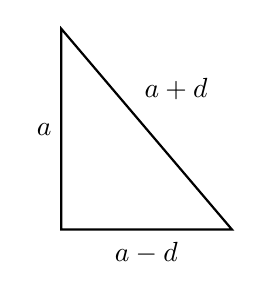
\begin{tikzpicture}[scale=0.85]
  \coordinate (T) at (0,3.0);
  \coordinate (L) at (0,0);
  \coordinate (R) at (2.55,0);
  \draw[thick] (T)--(L)--(R)--cycle;
  \node[left] at (0,1.5) {$a$};
  \node[below] at (1.27,-0.05) {$a-d$};
  \node[above right] at (1.1,1.8) {$a+d$};
\end{tikzpicture}
